%------------------------------------------------------------------------
%Editar Diplomado
\hypertarget{cv:eliminarTermino}{\section{Eliminar Término de Glosario}} \label{sec:eliminarTermino}

	Esta funcionalidad le permitirá eliminar un término innecesario o incorrecto. Para eliminar un término es necesario que no se encuentre asociado a casos de uso.

		\subsection{Procedimiento}

			%Pasos de procedimiento
			\begin{enumerate}
	
			\item Oprima el botón \IUBotonEliminar{} de un registro existente de la pantalla \ref{fig:GestionarGlosario} ''Gestionar Términos de Glosario''.
	
			\item Se mostrará el mensaje \ref{fig:confirmaEliminaTermino} sobre la pantalla \ref{fig:GestionarGlosario} ''Gestionar Términos de Glosario''.
			
			%Pantalla
			\begin{figure}[htbp!]
				\begin{center}
					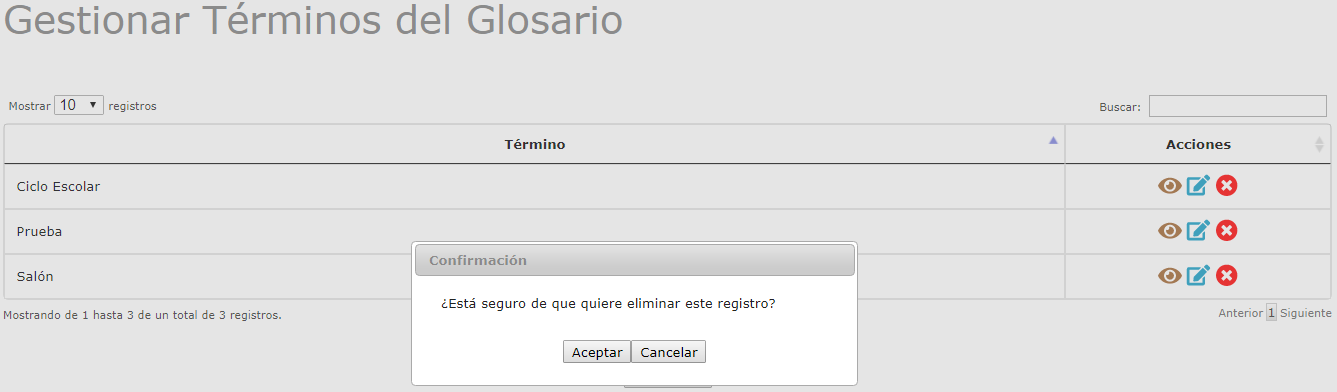
\includegraphics[scale=0.5]{roles/lider/glosario/pantallas/IU6-3MSG10}
					\caption{MSG de Confirmación}
					\label{fig:confirmaEliminaTermino}
				\end{center}
			\end{figure}
						
			\item Oprima el botón \IUAceptar.
			
			\item Se mostrará el mensaje \ref{fig:terminoEliminado} en la pantalla \ref{fig:GestionarGlosario} ''Gestionar Términos de Glosario''.
			
			\begin{figure}[htbp!]
				\begin{center}
					
\includegraphics[scale=0.5]{roles/lider/glosario/pantallas/IU6-3MSG1}
					\caption{MSG: Término Eliminado}
					\label{fig:terminoEliminado}
				\end{center}
			\end{figure}
			\end{enumerate}